%%%%%%%%%%%%%%%%%%%%%%%%%%%%%%%%%%%%%%%%%%%%%%%%%%%%%%%%%%%%%%%%
%%                                                            %%
%%   essentialsOfLatin, Italian translation 2017              %%
%%                                                            %%
%% From:  Henry C. Pearson, Essentials Of Latin For Beginners %%
%%        (1915, New York, American Book Company)             %%
%%                                                            %%
%%    https://archive.org/details/essentialslatin04peargoog   %%
%%                                                            %%
%% Translated by g.p.ciceri <gp.ciceri@gmail.com>             %%
%% ---------------------------------------------------------- %%
%% This translation is Licensed under                         %%
%% Creative Commons Attribution-ShareAlike 4.0 International  %%
%% https://creativecommons.org/licenses/by-sa/4.0/            %%
%%                                                            %%
%%%%%%%%%%%%%%%%%%%%%%%%%%%%%%%%%%%%%%%%%%%%%%%%%%%%%%%%%%%%%%%%

% āēīōū
% ăĕĭŏŭ




\documentclass[nols]{tufte-handout}

%\geometry{showframe} % display margins for debugging page layout

\usepackage{fontspec}
\usepackage{ifxetex}
\setmainfont[Path=./fonts/palatino-linotype/, ItalicFont=palai.ttf, BoldFont=palab.ttf]{pala.ttf}


% \defaultfontfeatures{Mapping=tex-text}
% \setromanfont[Path=./fonts/TeX-Gyre-Schola/,Mapping=tex-text]{TeX Gyre Schola}
% \setsansfont[Path=./fonts/TeX-Gyre-Heros/,Scale=MatchLowercase,Mapping=tex-text]{TeX Gyre Heros}
% \setmonofont[Path=./fonts/TeX-Gyre-Cursor/,Scale=MatchLowercase]{TeX Gyre Cursor}

\usepackage{lipsum}
\usepackage{url}
\usepackage{longtable}
\usepackage{stackengine}

\usepackage{graphicx} % allow embedded images
  \setkeys{Gin}{width=\linewidth,totalheight=\textheight,keepaspectratio}
  \graphicspath{{graphics/}} % set of paths to search for images
\usepackage{amsmath}  % extended mathematics
\usepackage{booktabs} % book-quality tables
\usepackage{units}    % non-stacked fractions and better unit spacing
\usepackage{multicol} % multiple column layout facilities
\usepackage{lipsum}   % filler text
\usepackage{fancyvrb} % extended verbatim environments
  \fvset{fontsize=\normalsize}% default font size for fancy-verbatim environments

% Standardize command font styles and environments
\newcommand{\doccmd}[1]{\texttt{\textbackslash#1}}% command name -- adds backslash automatically
\newcommand{\docopt}[1]{\ensuremath{\langle}\textrm{\textit{#1}}\ensuremath{\rangle}}% optional command argument
\newcommand{\docarg}[1]{\textrm{\textit{#1}}}% (required) command argument
\newcommand{\docenv}[1]{\textsf{#1}}% environment name
\newcommand{\docpkg}[1]{\texttt{#1}}% package name
\newcommand{\doccls}[1]{\texttt{#1}}% document class name
\newcommand{\docclsopt}[1]{\texttt{#1}}% document class option name
\newenvironment{docspec}{\begin{quote}\noindent}{\end{quote}}% command specification environment

% concetti morfosintattici
\usepackage{xspace} 
\newcommand{\noun}{\textsc{sostantivo}\xspace}
\newcommand{\nouns}{\textsc{sostantivi}\xspace}
\newcommand{\adject}{\textsc{aggettivo}\xspace}
\newcommand{\adjects}{\textsc{aggettivi}\xspace}
\newcommand{\gnumber}{\textsc{numero}\xspace}
\newcommand{\gnumbers}{\textsc{numeri}\xspace}
\newcommand{\gender}{\textsc{genere}\xspace}
\newcommand{\genders}{\textsc{generi}\xspace}
\newcommand{\gcase}{\textsc{caso}\xspace}
\newcommand{\gcases}{\textsc{casi}\xspace}
\newcommand{\tense}{\textsc{tempo}\xspace}
\newcommand{\mood}{\textsc{modo}\xspace}
\newcommand{\gverb}{\textsc{verbo}\xspace}
\newcommand{\gverbs}{\textsc{verbi}\xspace}
\newcommand{\adjective}{\textsc{aggettivo}\xspace}
\newcommand{\nom}{\textsc{nom}\xspace}
\newcommand{\gen}{\textsc{gen}\xspace}
\newcommand{\dat}{\textsc{dat}\xspace}
\newcommand{\acc}{\textsc{acc}\xspace}
\newcommand{\voc}{\textsc{voc}\xspace}
\newcommand{\abl}{\textsc{abl}\xspace}
\newcommand{\gexit}{\textsc{uscita}\xspace}
\newcommand{\gexits}{\textsc{uscite}\xspace}
\newcommand{\declinazione}{\textsc{declinazione}\xspace}
\newcommand{\masc}{\textsc{maschile}\xspace}
\newcommand{\femm}{\textsc{femminile}\xspace}
\newcommand{\neut}{\textsc{neutro}\xspace}

\newcommand{\indic}{\textsc{indicativo}\xspace}
\newcommand{\imper}{\textsc{imperativo}\xspace}
\newcommand{\gcong}{\textsc{congiuntivo}\xspace}
\newcommand{\ott}{\textsc{ottativo}\xspace}
\newcommand{\partic}{\textsc{participio}\xspace}
\newcommand{\infin}{\textsc{infinito}\xspace}

\newcommand{\pres}{\textsc{presente}\xspace}
\newcommand{\imperf}{\textsc{imperfetto}\xspace}
\newcommand{\aor}{\textsc{aoristo}\xspace}
\newcommand{\fut}{\textsc{futuro}\xspace}
\newcommand{\perf}{\textsc{perfetto}\xspace}
\newcommand{\pperf}{\textsc{piuccheperfetto}\xspace}

\newcommand{\sing}{\textsc{singolare}\xspace}
\newcommand{\plur}{\textsc{plurale}\xspace}
\newcommand{\dual}{\textsc{duale}\xspace}

\newcommand{\si}{\textsc{sing}\xspace}
\newcommand{\pl}{\textsc{plur}\xspace}
\newcommand{\du}{\textsc{dual}\xspace}

\newcommand{\att}{\textsc{attivo}\xspace}
\newcommand{\med}{\textsc{medio}\xspace}
\newcommand{\pass}{\textsc{passivo}\xspace}
\newcommand{\medpass}{\textsc{medio-passivo}\xspace}

\newcommand{\AC}{\textsc{a.C.}\xspace}
\newcommand{\DC}{\textsc{d.C.}\xspace}

% italianitudini
\renewcommand{\figurename}{Figura}
\renewcommand{\tablename}{Tabella}
\renewcommand{\contentsname}{Indice}

% fix per un qualche problema
\ifxetex
  \newcommand{\textls}[2][5]{%
    \begingroup\addfontfeatures{LetterSpace=#1}#2\endgroup
  }
  \renewcommand{\allcapsspacing}[1]{\textls[15]{#1}}
  \renewcommand{\smallcapsspacing}[1]{\textls[10]{#1}}
  \renewcommand{\allcaps}[1]{\textls[15]{\MakeTextUppercase{#1}}}
  \renewcommand{\smallcaps}[1]{\smallcapsspacing{\scshape\MakeTextLowercase{#1}}}
  \renewcommand{\textsc}[1]{\smallcapsspacing{\textsmallcaps{#1}}}
\fi

% too many float...
\extrafloats{100}

\title{Essentials Of Latin. Elementi di Latino. \newline Lezione XIX - Lezione di lettura e traduzione.}

\author[gpciceri]{a cura di Milagathòs: Milo's help to enjoy humanities.}

\date{18 Gennajo 2017} % without \date command, current date is supplied


\begin{document}

\maketitle% this prints the handout title, author, and date

\begin{marginfigure}[-2.5cm]
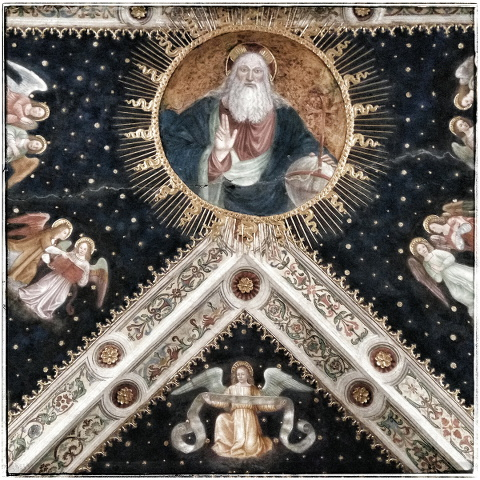
\includegraphics{smallthumb-lesson_XI.jpeg}
\setfloatalignment{b}
\end{marginfigure}


\begin{abstract}
\noindent
Queste lezioni riprendono il testo introduttivo al Latino di Pearson\cite{pearson1915}, del quale seguono la numerazione; la struttura di ogni lezione è piuttosto regolare: inizia con \textsc{cenni di morfologia e di sintassi latina}, seguita da un \textsc{piccolo vocabolario} per il lessico; ci sono infine vari \textsc{esercizi di traduzione e di composizione} latina.

\bigskip
\noindent
Lezione XIX: lezione di lettura e traduzione. Giulio Cesare, la Guerra con gli Elvezi. Suggerimenti per la traduzione.
\end{abstract}

%\printclassoptions

\newthought{134. Caio Giulio Cesare.} Giulio Cesare è il personaggio principale della storia di roma. La sua grandezza non è solo militare, come generale, ma anche politica, come oratore e statista. 

Nacque il 12 Luglio del 100 \AC, in una famiglia aristocratica di antica tradizione, ma sin dalla gioventù parteggò per il partito democratico. 

Dopo aver ricoperto vari incarici politici minori, all'età di quarantuno anni fu eletto console e formò un'alleanza politica con Pompeo e Crasso, conosciuta come \textit{Primo Triumvirato}. L'anno successivo gli fu assegnato il governo della Gallia, ed è la conquista di questo territorio che egli descrive nei suoi \textit{Commentarii}. Questi Commentari alle Guerre Galliche sono stati letti nelle scuole per centinaia d'anni, e testimoniano senza dubbio la grandezza di Cesare anche come scrittore.

Dopo aver passato otto anni in Gallia, gli fu ordinato dal Senato - per la gelosia di Pompeo - di sciogliere il suo esercito. Cesare rifiutò di obbedire e, attraversato il Rubicone, si avviò con una legione per diventare signore di Roma. Nella guerra civile che seguì, Pompeo, al comando delle forze armate senatoriali, venne sconfitto. Questo lasciò Cesare a capo del governo di Roma. Come Dittatore e Imperatore\sidenote{in senso, valido nella repubblica di Roma pre-imperiale, di comandante militare} perpetuo stabilì molte riforme, riforme che mostrano le sue capacità di statista. Tuttavia vi erano molti romani cui non piaceva il potere di Cesare: venne ordita una cospirazione, Cesare venne assassinato il 15 MArzo del 44 \AC. 

\newthought{135. La Guerra contro gli Elvezi.} Gli Elvezi erano popolazioni di origini celtiche che abitavano quasi tutto il territorio dell'attuale Svizzera.

Nell'anno 58 \AC, sotto il comando di capi ambiziosi, gli Elvezi decisero di lasciare le loro dimore e di occupare territori più fertili a Sud-Ovest, vicini alla allora Provincia Romana in Gallia. È a questa sollevazione degli Elvezi che Cesare dedica i primi trenta capitoli del suo primo libro dei Commentari alle Guerre Galliche. Dopo due battaglie gli Elvezi, battuti da Cesare, vennero costretti a ritornare nei territori da cui provenivano.

Le lezioni di lettura e traduzioni che seguono sono adattate dai primi dieci capitoli del racconto di Cesare di questa guerra contro gli Elvezi.

\newthought{136. Suggerimenti per la traduzione.}
\begin{itemize}
\item[\textsc{1.}] Leggi il passaggio (la frase) varie volte, e riconosci sin dall'inizio tutti i significati già chiari.
\item[\textsc{2.}] Tenta di associare i termini sconosciuti a parole già conosciute.
\item[\textsc{3.}] Non cercare il significato di una parola nel vocabolario senza aver fatto ogni sforzo possibile per riconoscerlo altrimenti. Se invece hai cercato il significato sul vocabolario, prenditi il tempo che ti serve per memorizzarlo.
\item[\textsc{4.}] Nel tentare di cogliere il significato di un passaggio, segui passo passo l'ordine Latino delle parole\sidenote{puoi anche riconoscere il significato rintracciando all'inizio gli elementi essenziali della frase: verbo, soggetto e complementi diretti - questa tecnica, la \textit{costruzione italiana della frase latina}, può aiutare nei primi tentativi}, osservando in particolare le loro terminazioni.
\item[\textsc{5.}] Traduci\sidenote{in un secondo tempo, dopo aver effettuato una prima traduzione, in cui si capisca senza dubbi ogni significato grammaticale e sintattico del testo latino} in un Italiano chiaro e scorrevole.
\end{itemize}

\newpage

\begin{figure}[!h]
  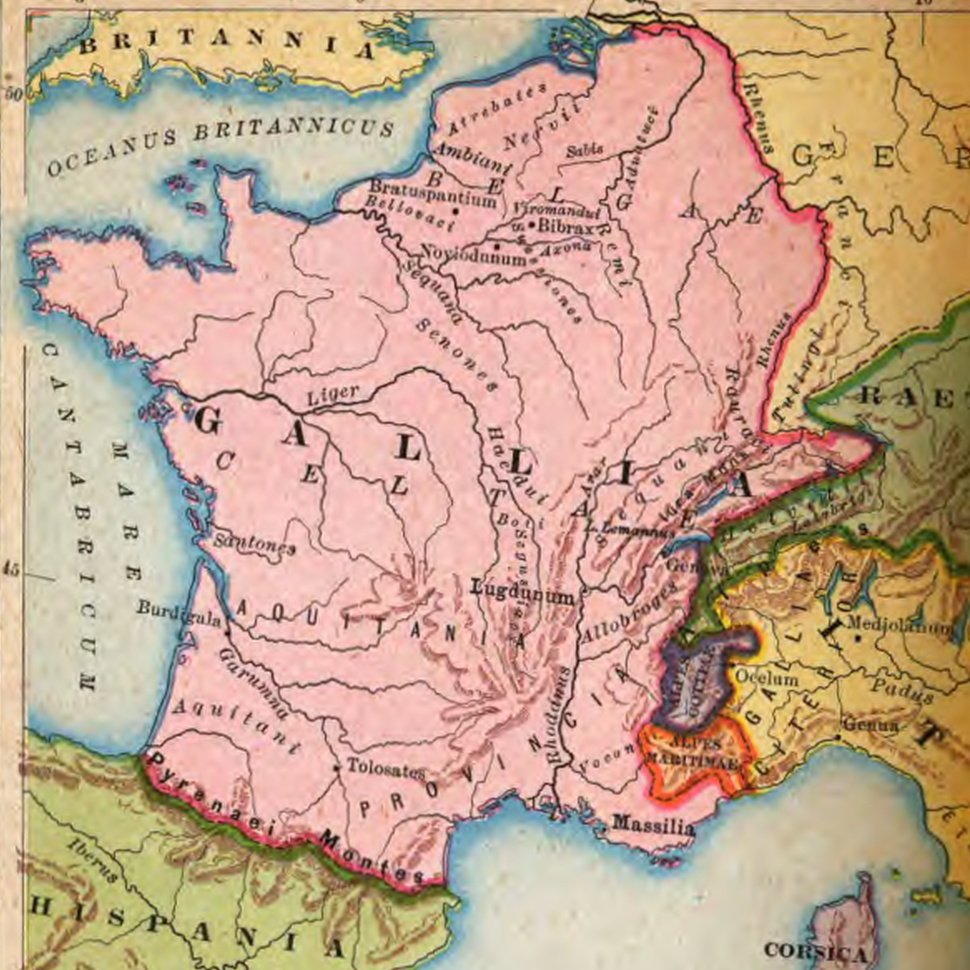
\includegraphics{mappaGalliaExEssentialsOfLatinDetail.jpeg}
  \caption{Mappa della Gallia (da Essentials of Latin}
  \label{fig:textfig}
  %\zsavepos{pos:textfig}
  %\setfloatalignment{b}
\end{figure}

\newthought{137. Lettura.} Capitolo I, \textsc{Descrizione della Gallia}.

Belgae\sidenote{vedi mappa} et Aquitani et Celtae Galliam incolunt\sidenote{indicativo presente, terza persona plurale, attivo, di \textbf{incolo}: \textit{essi abitano}. Puoi intuire il suo significato dalla parola \textbf{incola}?}. romani Celtas Gallos appellant. Belgae sunt fortissimi (\textit{i più coraggiosi}) et cum Germanis saepe pugnant. Helvetii sunt Celtarum fortissimi, quod (\textit{poiché}) cum Germanis continenter pugnant. Aquitania a Garumna flumine ad Pyrenaeos montes et ad eam (\textit{quella}) partem Oceani quae (\textit{la quale}) est ad Hispaniam pertinet.

\newthought{Nota.} Impara il paradigma (le parti pricipali) di tutti i verbi della prima e seconda coniugazione incontrati nel testo. Declina tutti i nomi e gli aggettivi.




\begin{figure}[!b]
  %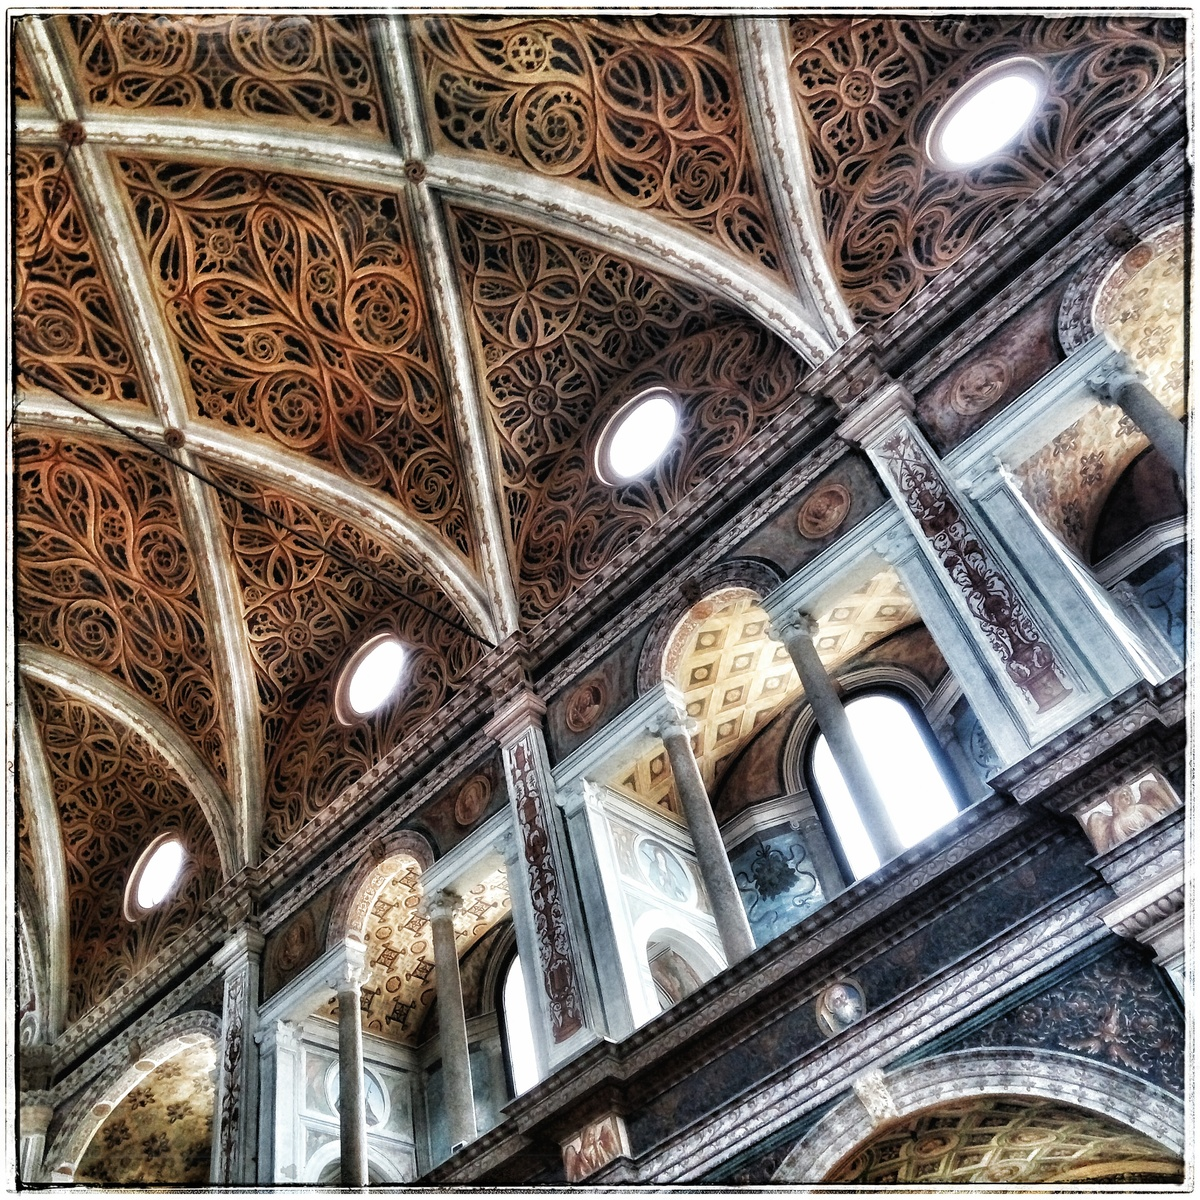
\includegraphics{thumb-lesson_XIX.jpeg}
  %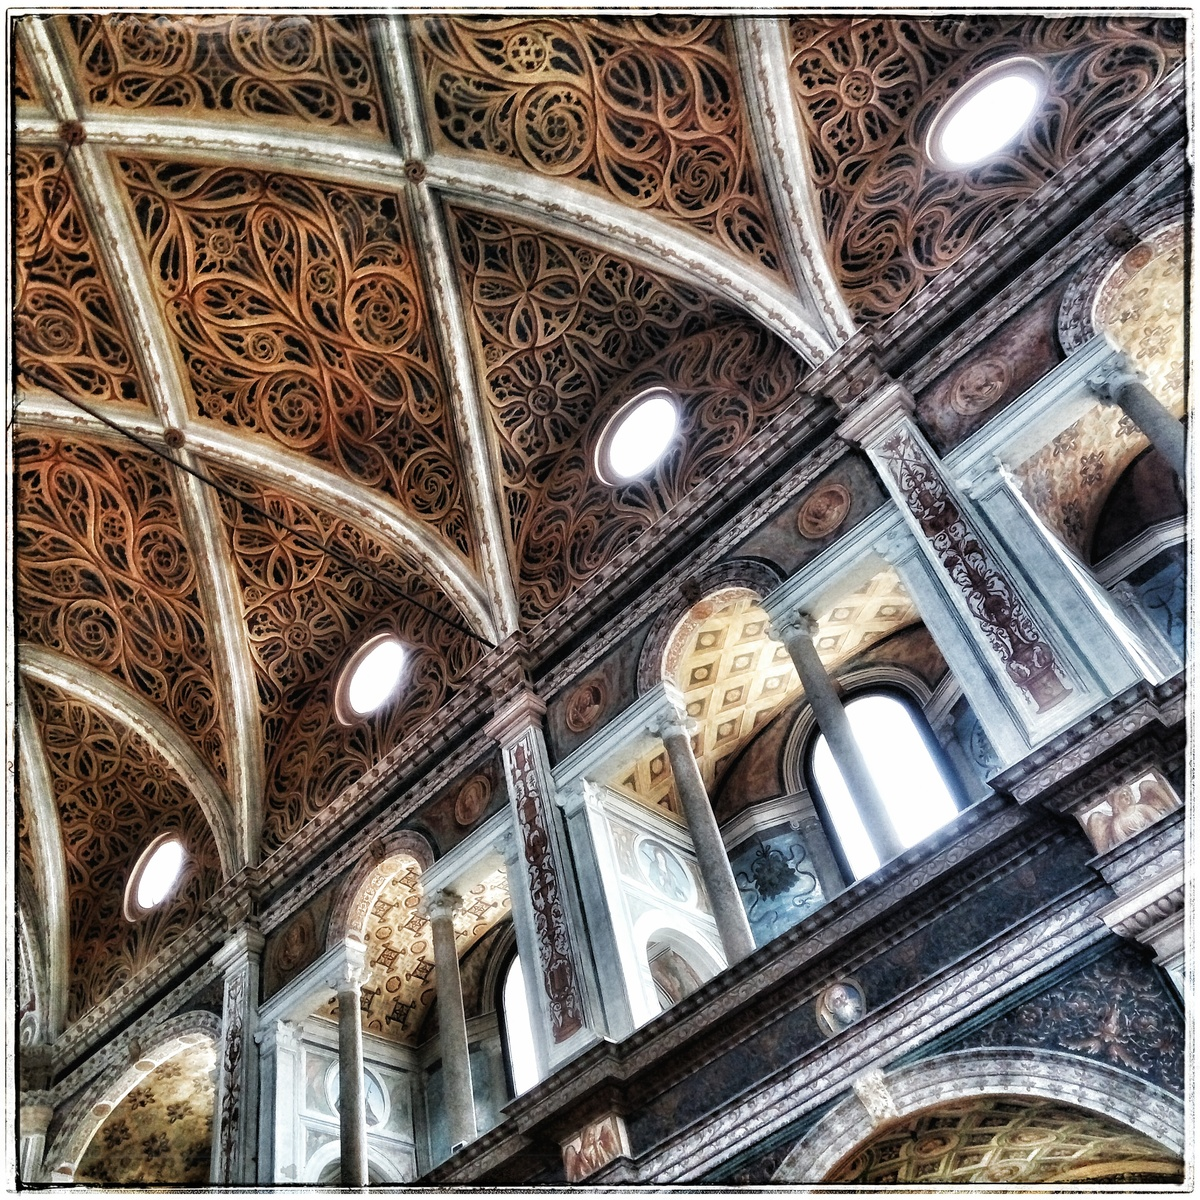
\includegraphics[width=0.9\linewidth]{thumb-lesson_XIX.jpeg}
  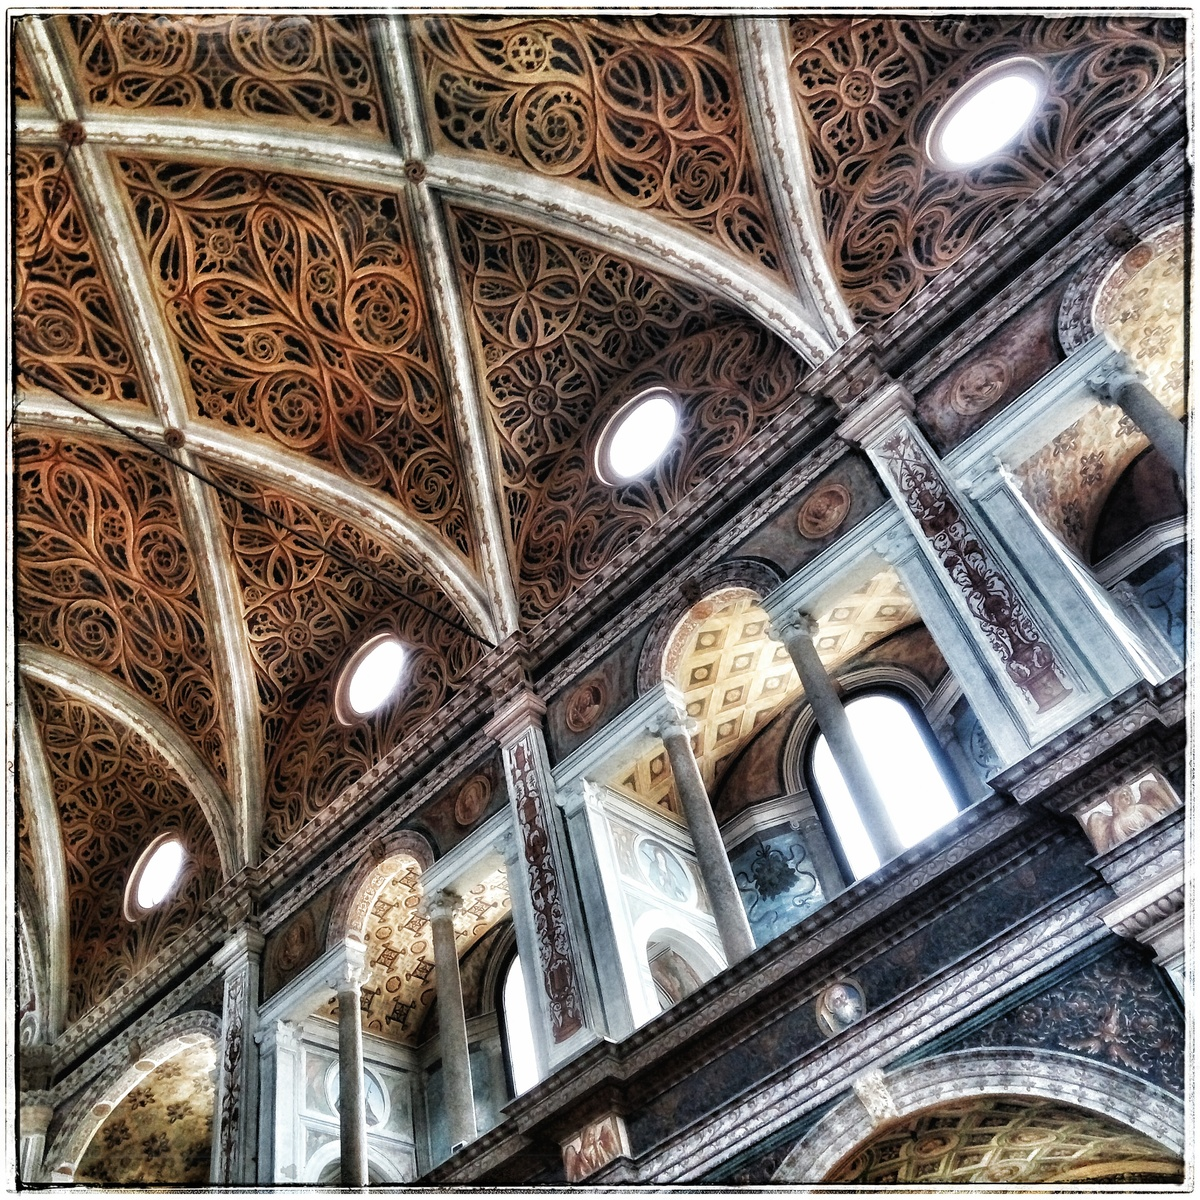
\includegraphics{thumb-lesson_XIX.jpeg}
  \caption{Milano: San Maurizio al Monastero Maggiore}
  \label{fig:textfig}
  %\zsavepos{pos:textfig}
  %\setfloatalignment{b}
\end{figure}
 

\nobibliography{latinBiblio}
\bibliographystyle{alpha}


\end{document}
